\chapterimage{supervisor.pdf}
\chapterimagecaption{\textit{The Lesson}  (1892) by George Goodwin Kilburne}

\chapter{Supervisor Relations}

    Your relationship with your supervisor is a very significant part of your graduate degree, as they will be the first point of contact for many of your concerns. Supervisors receive training before they take on students and should be prepared to address your questions and concerns effectively, however some of them may have done the training a long time ago and may be a little behind the times. \href{https://www.mcgill.ca/gradsupervision/supervisors/mcgill-expectations-graduate-supervision}{This page} on the McGill website provides a basic outline of what the expectations are for supervisors. 

    \section{Letter of Understanding and Progress Reports}\index{Letter of Understanding}\index{Progress Reports}
        
        To ensure accountability on both sides, McGill requires that you fill out "Progress Tracking" forms. Doctoral students are required to fill out a progress tracking form every year as a part of their degree requirements. Master's students are not explicitly required to fill out a progress tracking form as a part of their degree requirements, but they are heavily encouraged to do so.
        \\\\
        \href{https://www.mcgill.ca/gps/files/gps/gps_graduate_student_research_progress_tracking_report_2025_fillable.pdf}{This} is a link to the standard GPS progress tracking form. Broadly speaking the purpose of this is to write down a list of reasonable goals at the beginning of the year to provide accountability both for your supervisor and for you. You are evaluated on whether or not you have achieved the written goals at the next progress tracking meeting (next year), and the evaluation also involves a lengthy justification section (if your progress is unsatisfactory). This section requires your supervisory committee to reference specific aspects of your previous objectives section, and this should inform how you pick objectives when sitting down with your supervisor at the beginning of the year. GPS has \href{https://www.mcgill.ca/gradsupervision/supervisees/discussing-expectations}{this} webpage that is a little bit more detailed about the intention behind writing a letter of understanding.
        \\\\
        The department also provides a guidelines document (which appears to be a Faculty of Science document from 2022) \href{https://www.physics.mcgill.ca/grads/lou22.pdf}{here}. This document is much more specific about what exactly should be discussed at a progress tracking meeting, and has a list of suggestions for additional topics.

    \section{Switching Supervisors}
        It is possible that you may need to switch supervisors during your degree. This can happen for a number of reasons, and in the event that either you or your supervisor feel that you need to end the supervisory relationship your department chair will assist you in finding a new supervisor. GPS has \href{https://www.mcgill.ca/gps/files/gps/graduate_student_supervision_change_of_supervisor_guidelines_april_2026.pdf}{this} document, this is written for department chairs but it describes what the process would be like for you as well. GPS also has \href{https://www.youtube.com/watch?v=4IuLZEAB_aU&t=6s}{this} video going over some things to consider and how to go about the process. The video is also described at the bottom of \href{https://www.mcgill.ca/gradsupervision/supervisees/conflict-resolution}{this} webpage.

    \section{How to file complaints}\label{section:supercomp}
        If you are having difficulty with your supervisor, your first point of contact is the graduate program director (Nikolas Provatas). If this is not an avenue you feel comfortable taking or if you have already tried this without success, there are a number of other options that you can take. GPS provides \href{https://www.mcgill.ca/gradsupervision/supervisees/conflict-resolution}{this} webpage describing the avenues you have to pursue a complaint, along with the summarizing graphic below. The gist is that ideally you want to address the complaint locally first (i.e. with your supervisor, with the graduate program director, chair, or other professors in your department), then move up to more official avenues through the GPS and the university. There are a series of additional offices in the university that are able to help with conflict resolution which are listed on the right of the figure below.

        \begin{figure}[H]
            \centering
            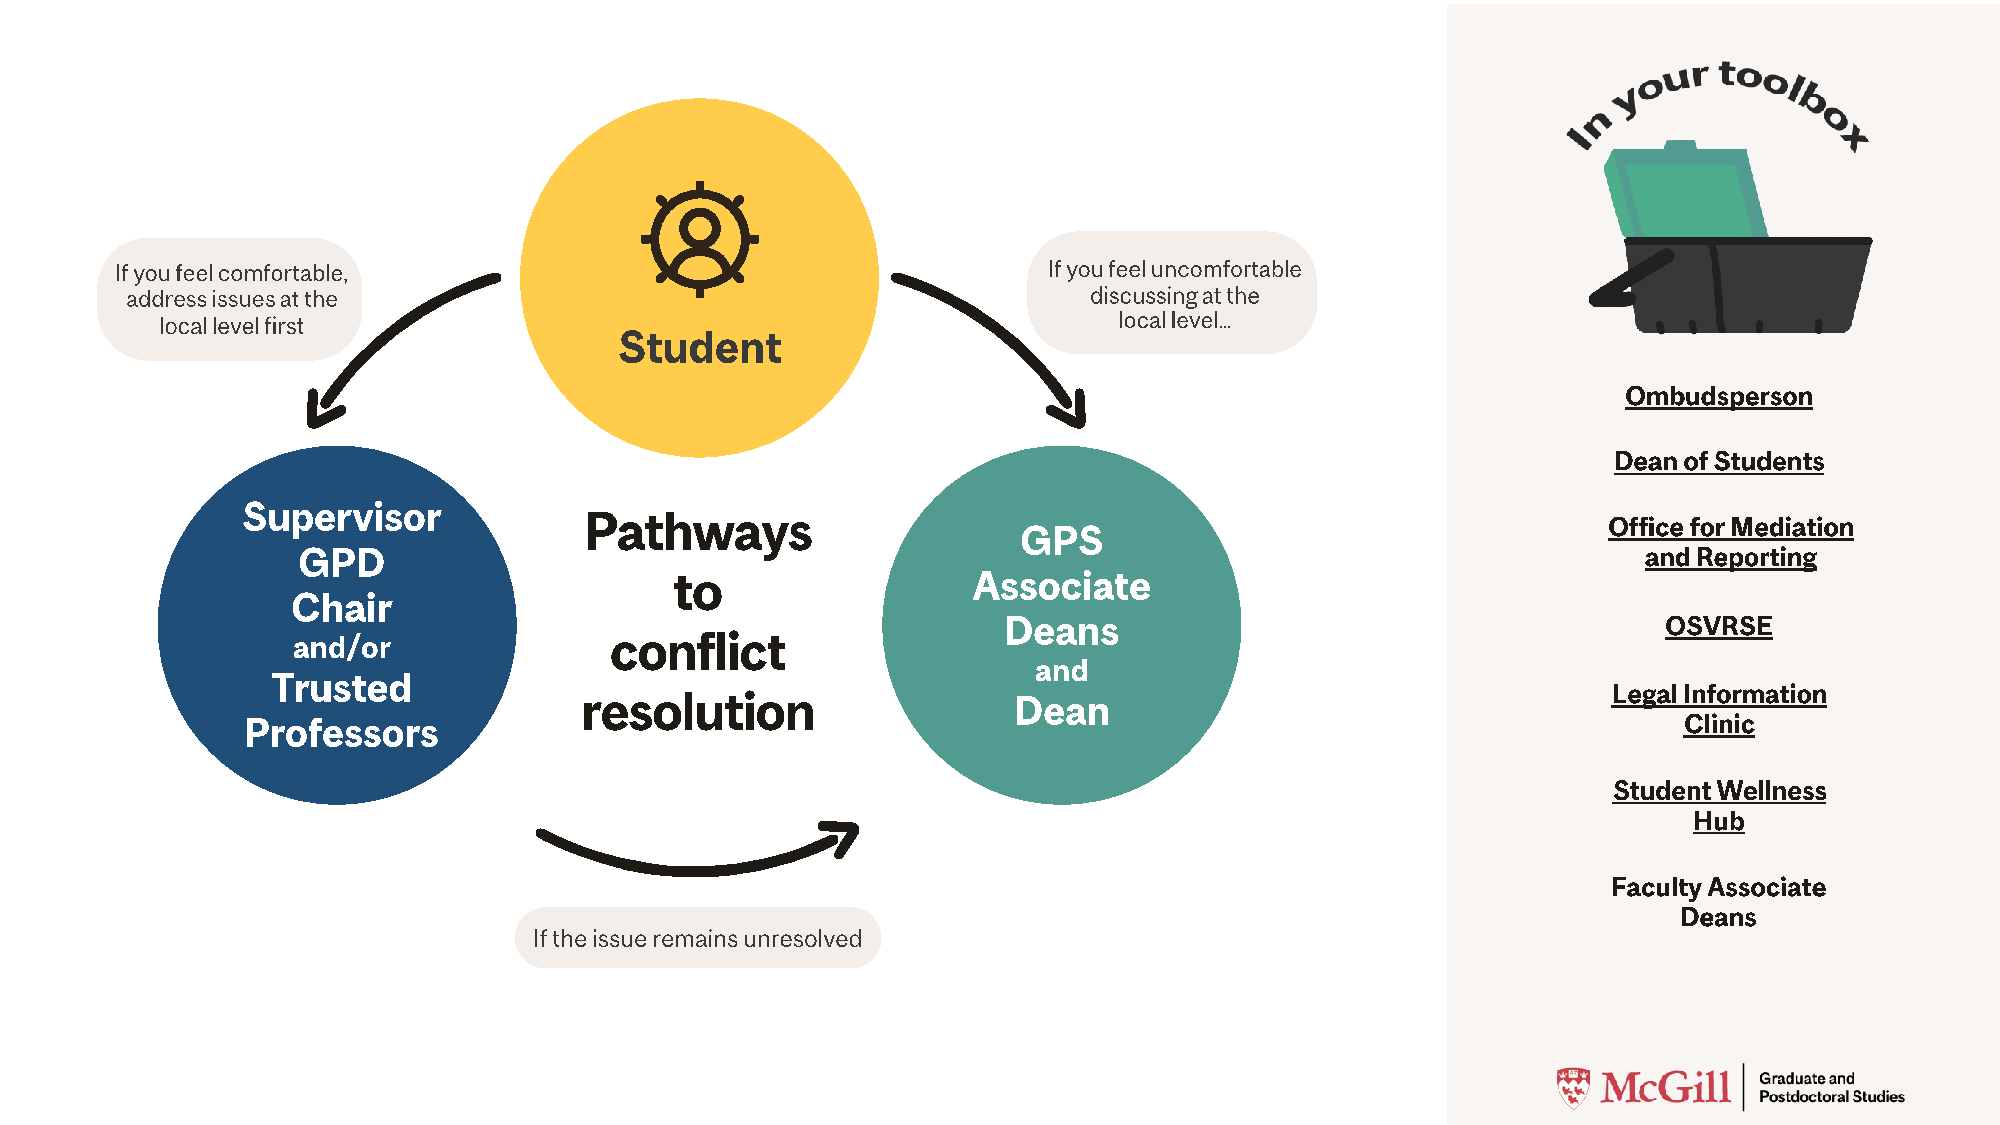
\includegraphics[width=0.95\columnwidth]{Pictures/conflict_resolution_flowchart.pdf}
        \end{figure}
        
        GPS also provides supervisors with \href{https://www.mcgill.ca/gradsupervision/supervisors/resolving-conflict}{this} webpage on resolving conflict, which can inform how you go about addressing a conflict with your supervisor before reaching out to the program director.